\chapter{NOGWs excited by tropopause depressions in a 2D plane}
\label{sec:resultsQ3D}
It is the goal of this chapter to address the second research question
\begin{tcolorbox}[]
    (R1) How sensitive are NOGWs from propagating tropopause depressions to the depression's 2D shape and to 2D properties of the stratospheric environment?
\end{tcolorbox}
\noindent and identify zonal and vertical properties of the tropopause and the stratospheric environment that significantly influence the appearance and propagation of NOGWs above propagating tropopause folds. \\
At first, section \ref{fig:q3D_referenceSim} presents the reference simulation for this sensitivity study and recapitulates important assumptions and properties of the simulations. Then three sections investigate variations of the GW activity in the stratosphere when changing the propagation speed of the tropopause fold (section \ref{sec:q3D-speed}), the zonal shape of the tropopause fold (section \ref{sec:q3D-shape}) and the vertical profile of the ambient wind or the Coriolis force (section \ref{sec:q3D-wind}). A short summary (section \ref{sec:q3D-summary}) completes this analysis. 

\section{The reference simulation}
\label{sec:resultsq3D-reference}
\begin{figure*}[t]
    \centering
    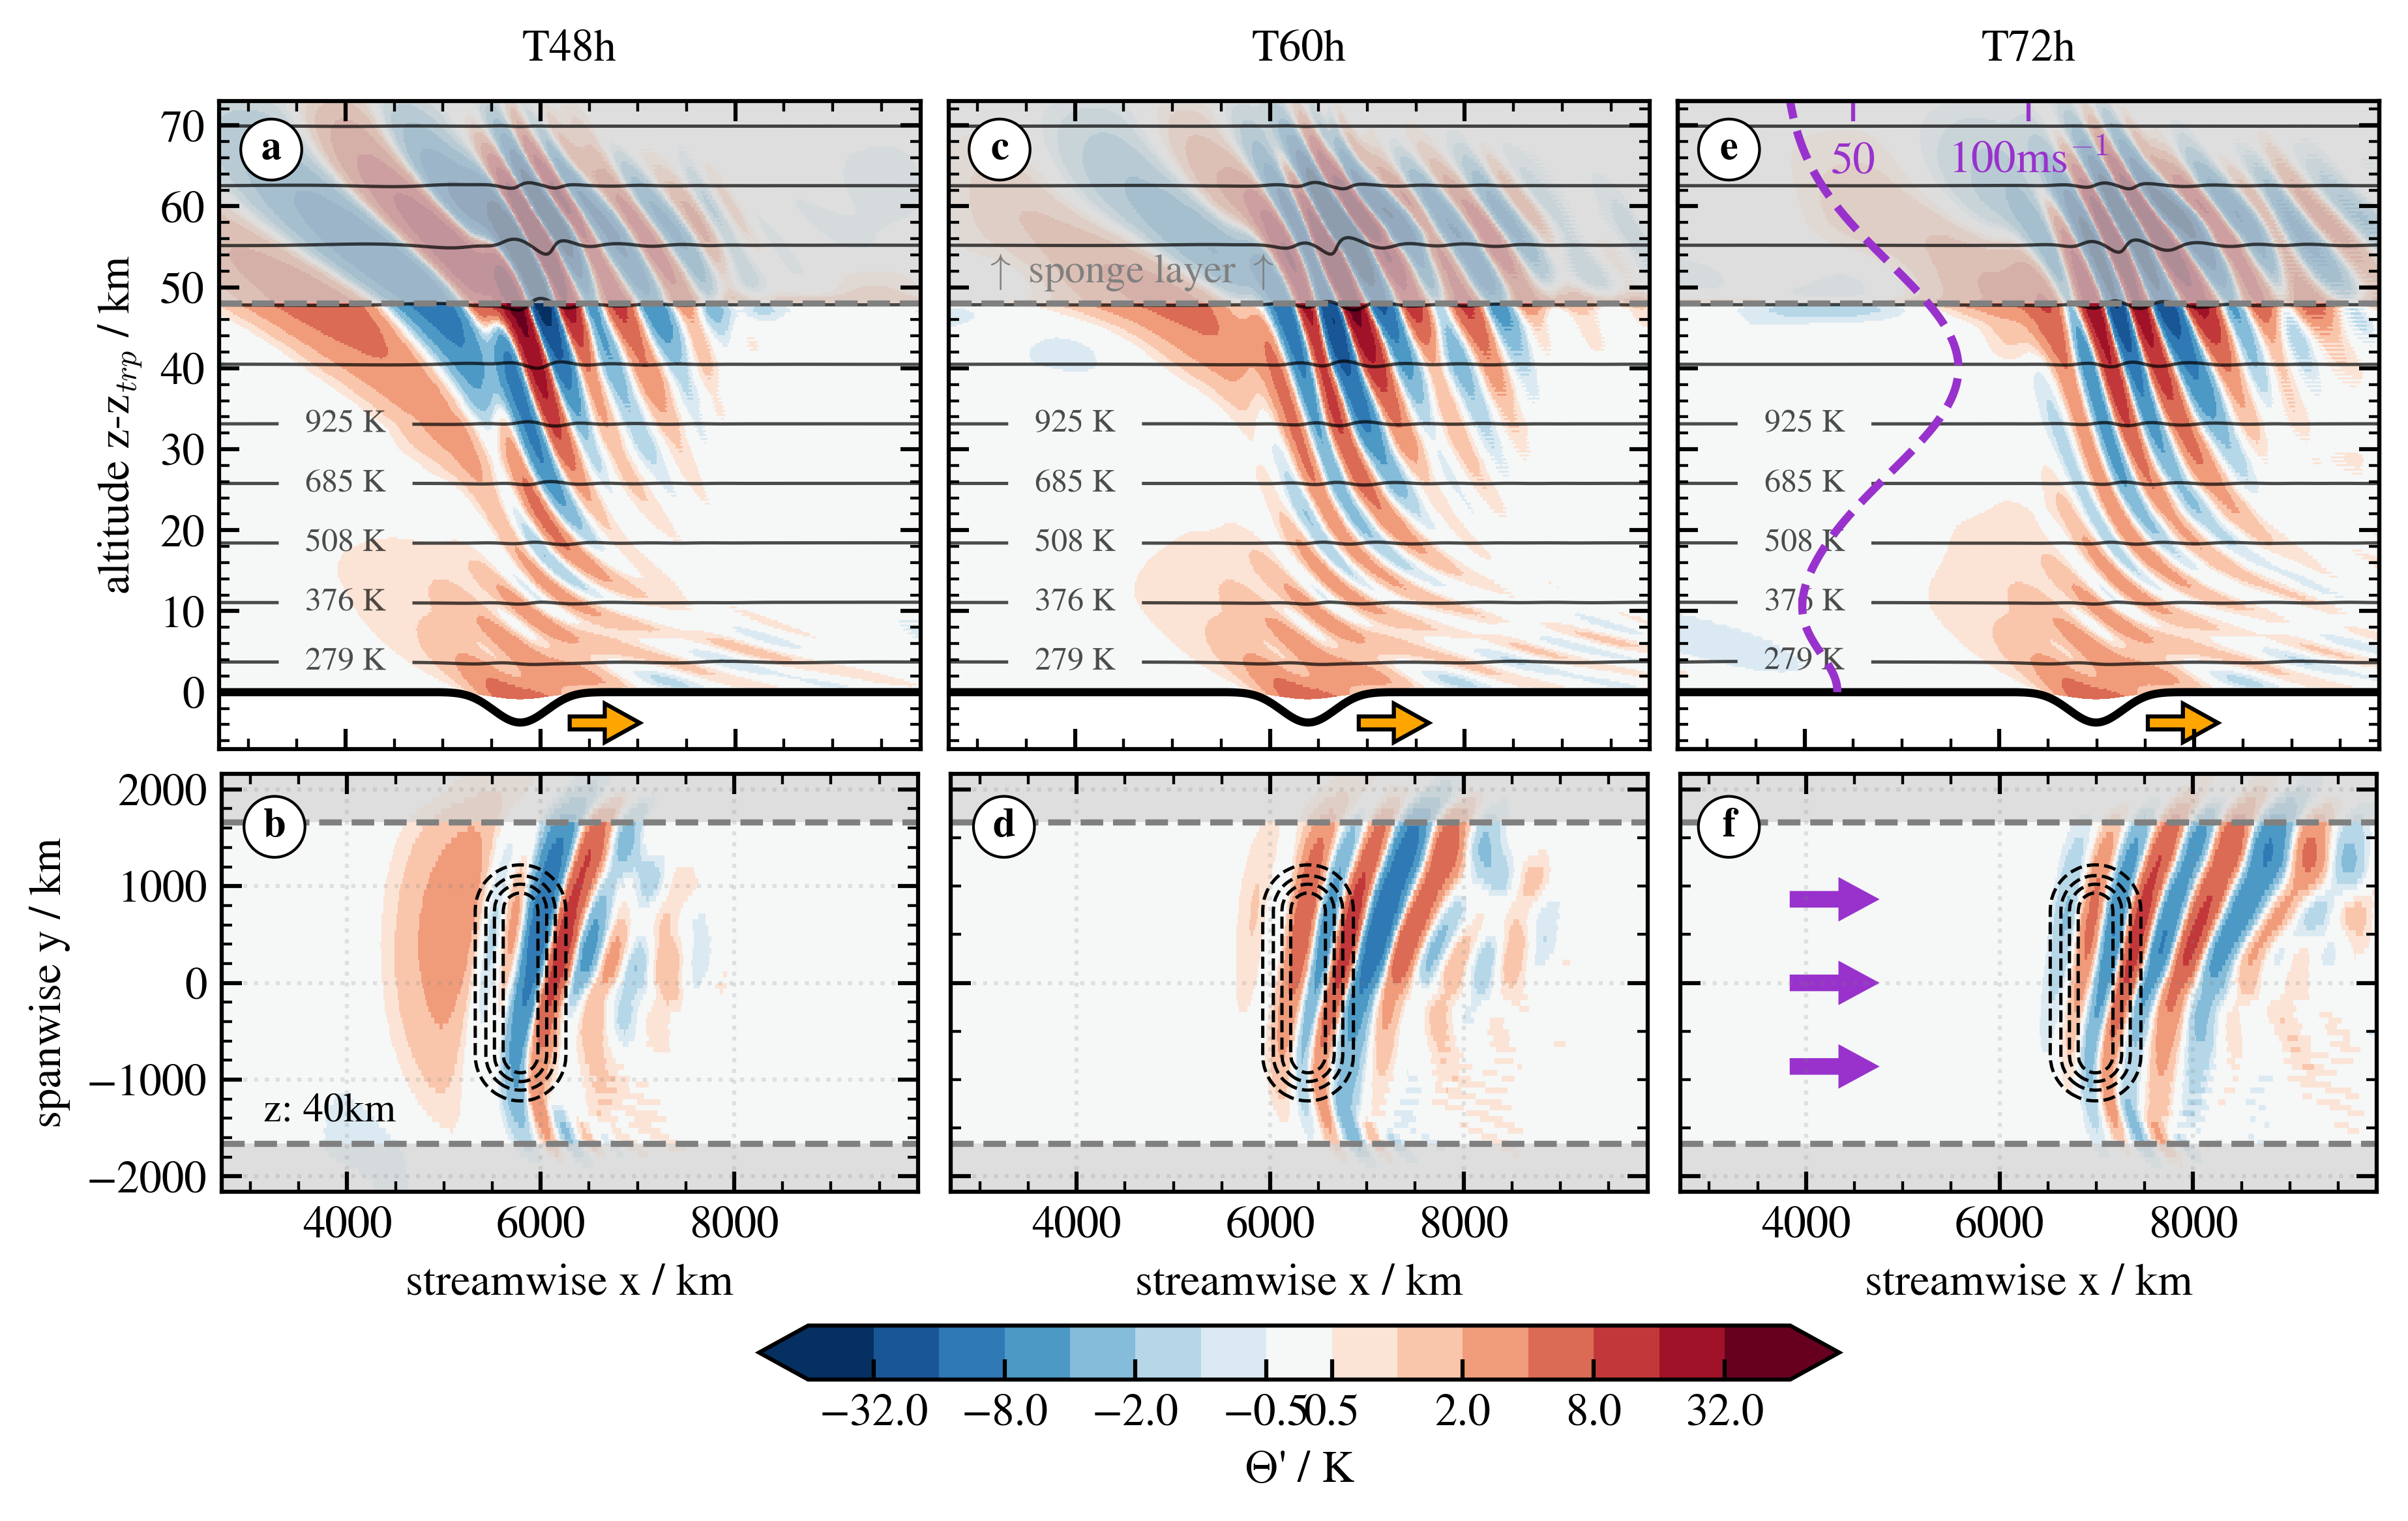
\includegraphics[width=0.99\textwidth]{figures_q3D/Q3D-th-referenceSim.png}
    \caption{Visualized is $\Theta'$ for three timesteps of the reference simulation in vertical cross sections (a), (c) and (e) for y=0 and horizontal cross sections (b), (d) and (f) \SI{40}{\kilo\meter} above the tropopause. The tropopause fold at the lower boundary moves with a constant speed $c_{tf}=\SI{13.88}{\meter\per\second}$ towards the right. Its height is exaggered by a factor of 5 and thin lines above represent constant potential temperature. The vertical ambient wind profile (purple line in (e)) is constant in meridional direction as indicated in (f). Dashed lines in the horizontal cross sections define the shape of the elongated fold and grey areas indicate sponge layers.}
    % of the sensitivity study
    \label{fig:q3D_referenceSim}
\end{figure*}
%
The model validation (section \ref{sec:linear-MWs}) showed that a correct integration of rotational (Coriolis) effects requires 3D simulations. Consequently, all simulations in this chapter are 3D though the following analysis focuses on the 2D plane at y=0. Figure \ref{fig:q3D_referenceSim} illustrates the reference simulation for the sensitivity study. As indicated in Figure \ref{fig:q3D_referenceSim}e and f, the background wind $u_e(z)$ only changes in the vertical direction and is constant in meridional direction. In a similar manner, the meridional shape of the lower boundary (dashed lines in horizonal cross sections) is constant in the center of the domain and only changes close to the sponge layers. The zonal shape of the transient boundary is prescribed by the cosine function (equation (\ref{equ:cosMtn})) and it propagates with a constant speed $c_{tf}=\SI{13.88}{\meter\per\second}$ in the direction of the arrows. To recap, the transient, impermeable and frictionless lower boundary mimics the tropopause or more precisely an isentrope just above the tropopause. This isentrope still dips above a tropopause fold, but it does not reach areas within the fold that are prone to increased mixing. For the reference simulation the half width of the fold is $L = \SI{300}{\kilo\meter}$ and the maximum depth of the fold is \SI{750}{\meter}. The ambient background atmosphere is isothermal (Bacmeister-Schoeberl Model described in section \ref{sec:ambient-profiles}) and follows the stratosphere setup from table \ref{tab:ambientProfiles} with a constant Brunt-Väisälä frequency $N=\SI{0.02}{\per\second}$. $f = \SI{-1.195e-4}{\per\second}$ refers to a latitude of $\SI{55}{\degree S}$ and maximum wind speeds of the tropopause and polar night jet are $u_{TPJ,max}=\SI{45}{\meter\per\second}$ and $u_{PNJ,max}=\SI{80}{\meter\per\second}$, respectively. \\
All simulations stick to $n_t$=\SI{4320}{timesteps} on a grid with (n$_z$,n$_y$,n$_x$)=(301,72,720) grid points and a constant resolution of dt=\SI{60}{\second} and (dz,dy,dx)=(\SI{250}{\meter},\SI{60}{\kilo\meter},\SI{15}{\kilo\meter}). Sponge layers in vertical and spanwise direction are indicated in Figure \ref{fig:q3D_referenceSim} and periodic boundaries are used streamwise to avoid a very wide domain due to the motion of the tropopause fold.
%
% limitations of these simulations...
%
\section{The influence of the fold's propagation speed}
\label{sec:q3D-speed}
\begin{figure*}[tbp]
    \centering
    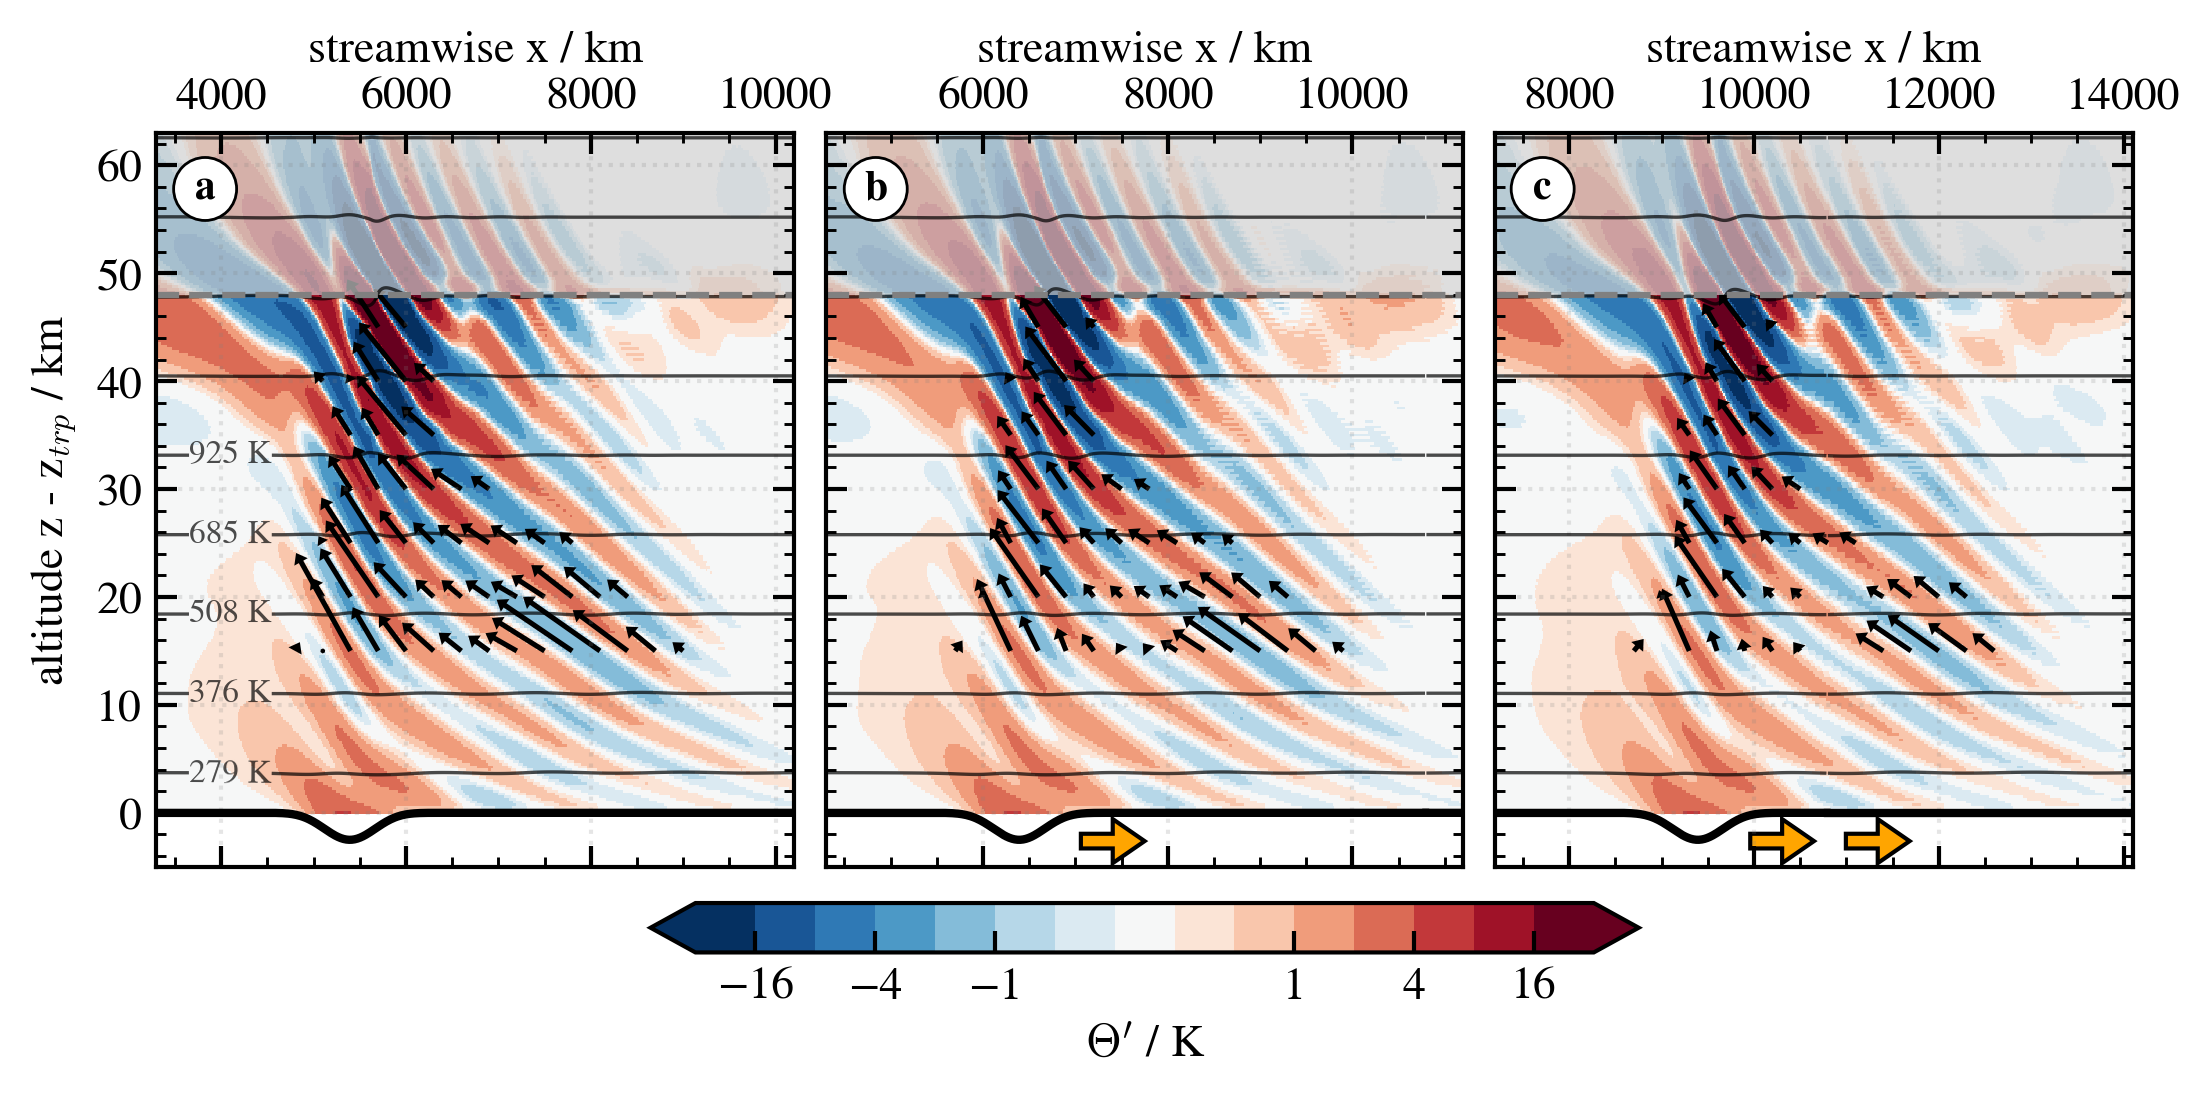
\includegraphics[width=0.99\textwidth]{figures_q3D/Q3D-TH-EF-ctropo.png}
    \caption{Shown are potential temperature perturbations $\Theta'$ overlayed by normalized vectors of \textbf{EF} for three different simulations with a constant background wind profile $u_e$ that corresponds to a $u_{e,MW}=\SI{31.12}{\meter\per\second}$. (a) represents the "MW case" with a stationary lower boundary. In (b) the tropopause fold moves with $c_{tf}$ and the backround wind is increased by $c_{tf}$. In (c) the tropopause fold moves with $2c_{tf}$ and again the backround wind is increased by $2c_{tf}$ with respect to (a). Note the different positions of the tropopause fold in streamwise direction after t=\SI{60}{\hour} and the strong similarity of all three simulations.}
    \label{fig:q3D_ctropo}
    % difference due to rising mountain?? 
\end{figure*}
We start with the propagation speed of the tropopause fold $c_{tf}$, because its relation to the background wind $u_e(z)$ is probably the most fundamental result of this chapter. Simulations with different $c_{tf}$ showed that the wave activity within a reference frame moving with the fold only depends on the relative difference between $u_e(z)$ and $c_{tf}$. Thus, it is possible to define a mountain wave wind speed
\begin{equation}
    u_{e,MW}(z) = u_e(z)-c_{tf}
    \label{equ:MW_forcing}
\end{equation}
that leads to an identical GW pattern with a stationary tropopause fold as in the propagating case. The complete vertical wind profile has to be reduced by $c_{tf}$ to achieve similar GWs. In other words, variations of the complete vertical profile $u_e(z)$ have a similar effect on the GW activity as variations of the fold's propagation speed. Figure \ref{fig:q3D_ctropo} visualizes an example showing three simulations with varying $u_e$ and $c_{tf}$, but a constant $u_{e,MW}=\SI{31.12}{\meter\per\second}$. The position of the tropopause fold after t=\SI{60}{\hour} is very different, but the GW field looks quite similar for all simulations. Minor differences in perturbations are most likely related to varying interactions with the vertical sponge layer due to $c_{tf}$. The energy flux \textbf{EF} overlayed in all three simulations (Figure \ref{fig:q3D_ctropo}) allows a similar conclusion. As expected, its direction is always parallel to the phase lines and the overall pattern for (a)-(c) in Figure \ref{fig:q3D_ctropo} is similar. Only magnitudes of \textbf{EF} vary slightly between simulations. \\
The conclusion of this finding might be quite instructive. Under the assumptions of the proposed excitation mechanism (tropopause fold mimics an obstacle for the stratospheric flow above like a mountain or valley at the surface) NOGWs above these propagating folds behave and propagate just like MWs within the reference frame of the propagating fold for $u_{e,MW}$. Therefore, known properties of MWs are transferable to NOGWs above tropopause folds, but nevertheless a concise investigation with a moving tropopause fold follows within the next sections and chapter \ref{sec:results3D}.
% Under the assumption of 
%
\section{The influence of the tropopause shape}
\label{sec:q3D-shape}
% This section is kept short. 
To simplify the qualitative analysis of parameter variations and also provide a quantitative overview on certain aspects, different simulations are primarily compared based on Figures \ref{fig:q3D_shape} and \ref{fig:q3D-wind}, which show vertical profiles of momentum and energy fluxes. This section focuses on Figure \ref{fig:q3D_shape} and the variation of the zonal width and the depth of the tropopause depression.

A smaller width of the depression naturally results in shorter horizontal wavelengths and, therefore, in higher momentum and energy fluxes as illustrated in (a)-(c) of Figure \ref{fig:q3D_shape}. This makes sense, because waves with smaller horizontal or vertical scales concentrate their energy in a smaller area. In addition, smaller wavelengths lead to a higher frequency and waves travel faster (e.g. \cite[]{gill_atmosphere-ocean_1982}). Both phenomena lead to higher momentum and energy fluxes. (a), for example, suggests that decreasing the zonal width by $\frac{1}{3}$ increases the angular momentum flux MF$_{x,ang}$ in the upper stratosphere ($z \approx \SI{30}{\kilo\meter}$) by a factor of 5-6 (purple dashed line vs. black solid line). Note that statements like "increasing" or "decreasing" will always refer to the amount of the fluxes independent of their sign. The sign indicates the direction of the flux. \\
In (b) EF$_z$ is about 6 times higher for $L=\SI{200}{\kilo\meter}$, too. As described in section \ref{sec:linear-MWs}, the Eliassen-Palm relation for rotating fluids from equation (\ref{equ:EP-relation-rotating}) states that MF$_{x,ang}$ and EF$_z$ are related via the background wind. A similar ratio between simulations for MF$_{x,ang}$ and EF$_z$ suggests that the EP relation is applicable. Furthermore, the vertical profile of the energy flux EF$_z$ nicely illustrates how wave energy is reduced in areas with negative shear (lower stratosphere) and produced in the positive shear of the PNJ (compare with Figure 6 of \textcite[]{eliassen_transfer_1960}). Physically, this variation of EF$_z$ can also be interpreted as a conversion of mean flow shear energy to wave energy flux (\cite[]{kruse_gravity_2015}). From a relative point of view, the production of EF$_z$ due to the PNJ (positive shear between 15 and \SI{40}{\kilo\meter}) is similar for $L=\SI{200}{\kilo\meter}$ and $L=\SI{300}{\kilo\meter}$. It is approximately \SI{70}{\percent}.

\begin{figure*}[t]
    \centering
    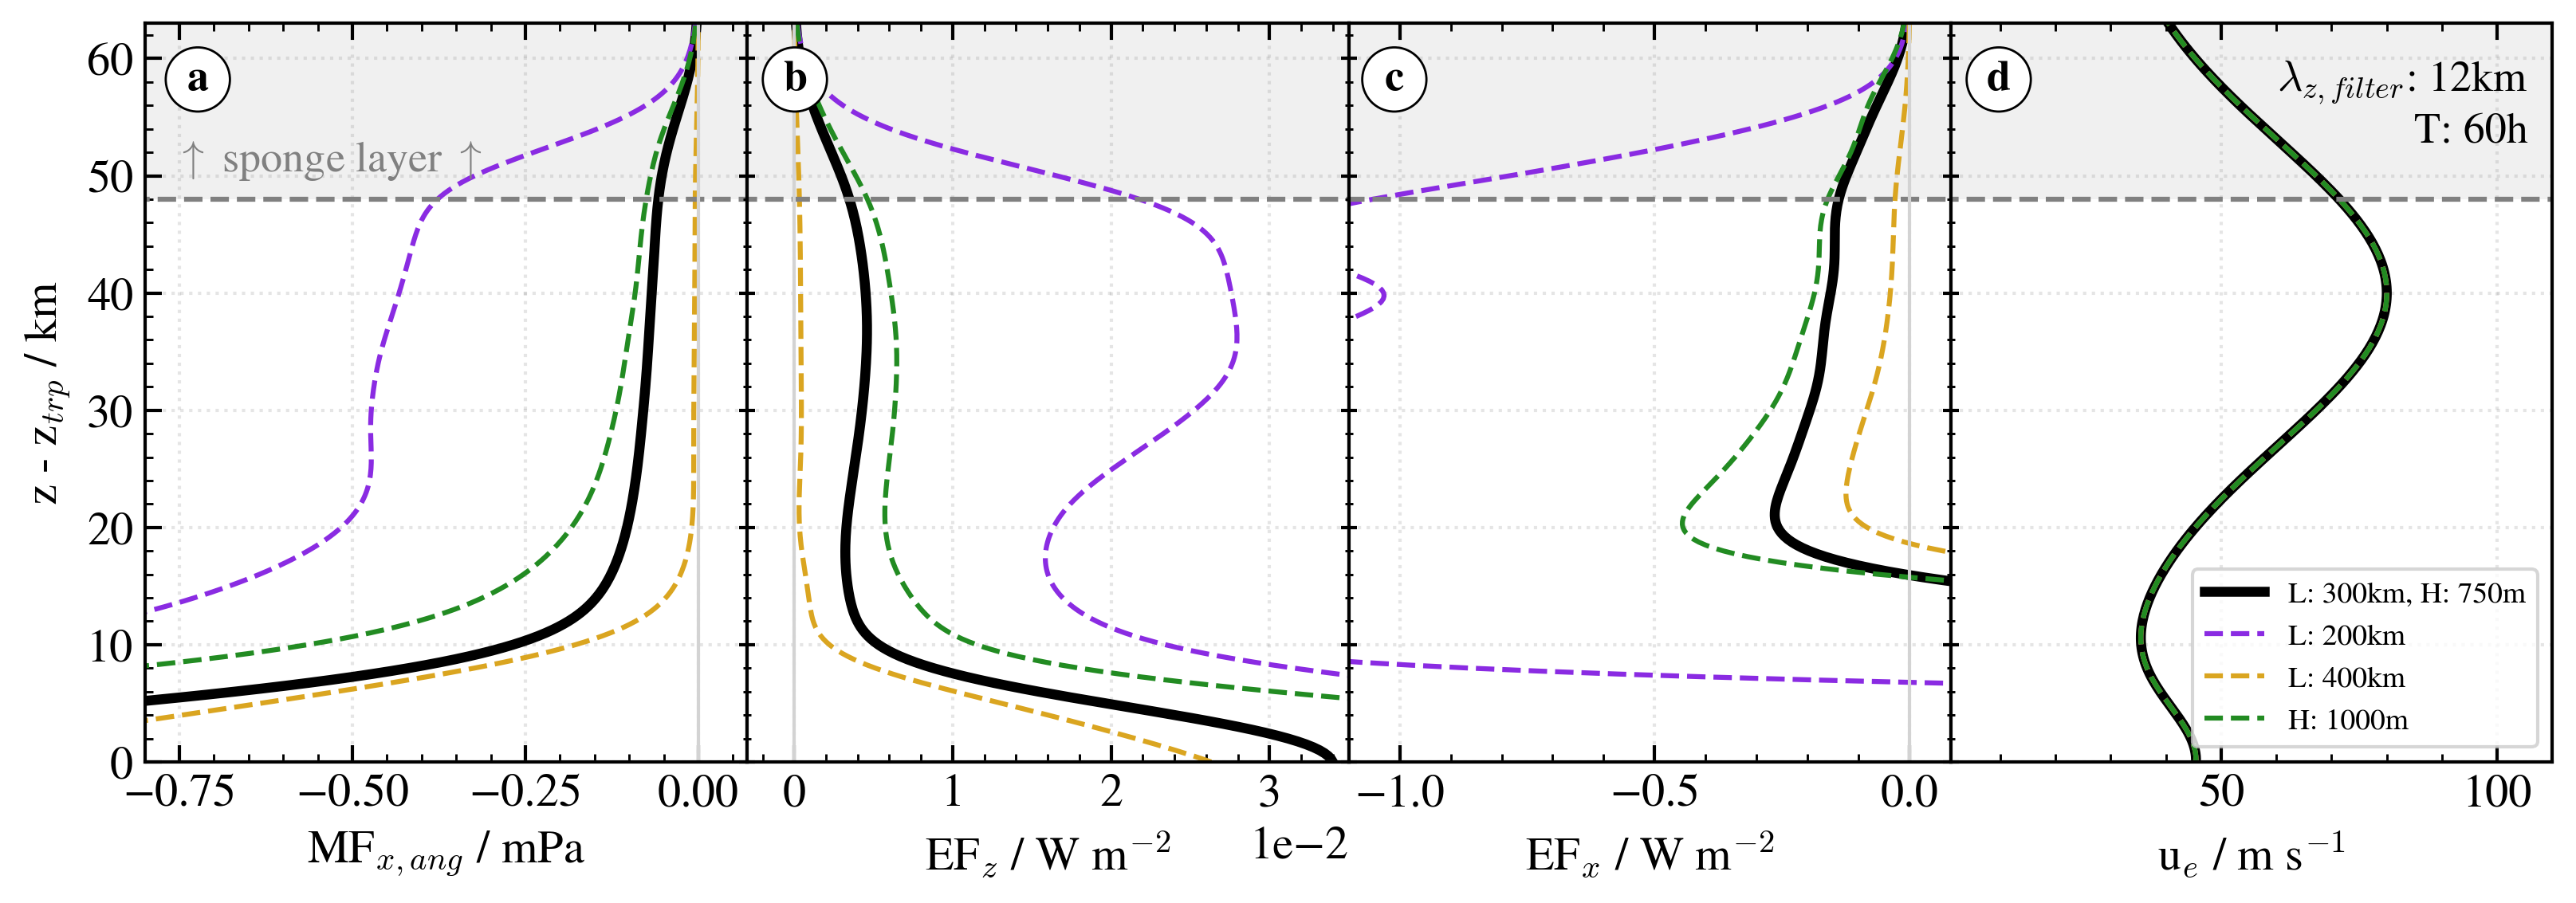
\includegraphics[width=0.99\textwidth]{figures_q3D/TD-zprofiles-translbq3D_shape-T60h-avg.png}
    \caption{Vertical profiles of zonal averages for the vertical flux of zonal angular momentum MF$_{x,ang}$ (a), the vertical energy flux EF$_z$ (b), the zonal energy flux EF$_x$ (c) and the ambient wind $u_e$ (d) for different simulations with a propagating tropopause fold. The thick black solid line represents the reference simulation from Figure \ref{fig:q3D_referenceSim} and dashed lines refer to variations of this simulation as stated in the legend of (d). All profiles are filtered in the vertical with a cutoff wavelength $\lambda_{z,filter}=\SI{12}{\kilo\meter}$. In this figure, all simulations utilize the same wind profile $u_e(z)$.}
    \label{fig:q3D_shape}
\end{figure*}
A larger depth of the tropopause fold increases all momentum and energy fluxes in Figure \ref{fig:q3D_shape}, because larger deflections at the tropopause increase perturbation amplitudes throughout the stratosphere. However, horizontal scales of the GWs, propagation speeds or the wave regime in general are not affected. The horizontal energy flux EF$_x$ in (c) depicts this most clearly. While variations of the depression width lead to different heights for the sign change of EF$_x$, the simulation with an increased depression depth has an identical height for the transition from positive to negative values of EF$_x$ as the reference simulation. The reason for this transition of EF$_x$ in the lower stratosphere is not fully understood. It is also observed for low frequency waves or IGWs and a constant wind profile during the model validation in section \ref{sec:linear-MWs}. Therefore, it seems to be related to rotational effects.
% 3D nature of IGWs and
%
\section{The influence of the stratospheric environment}
\label{sec:q3D-wind}
\begin{figure*}[t]
    \centering
    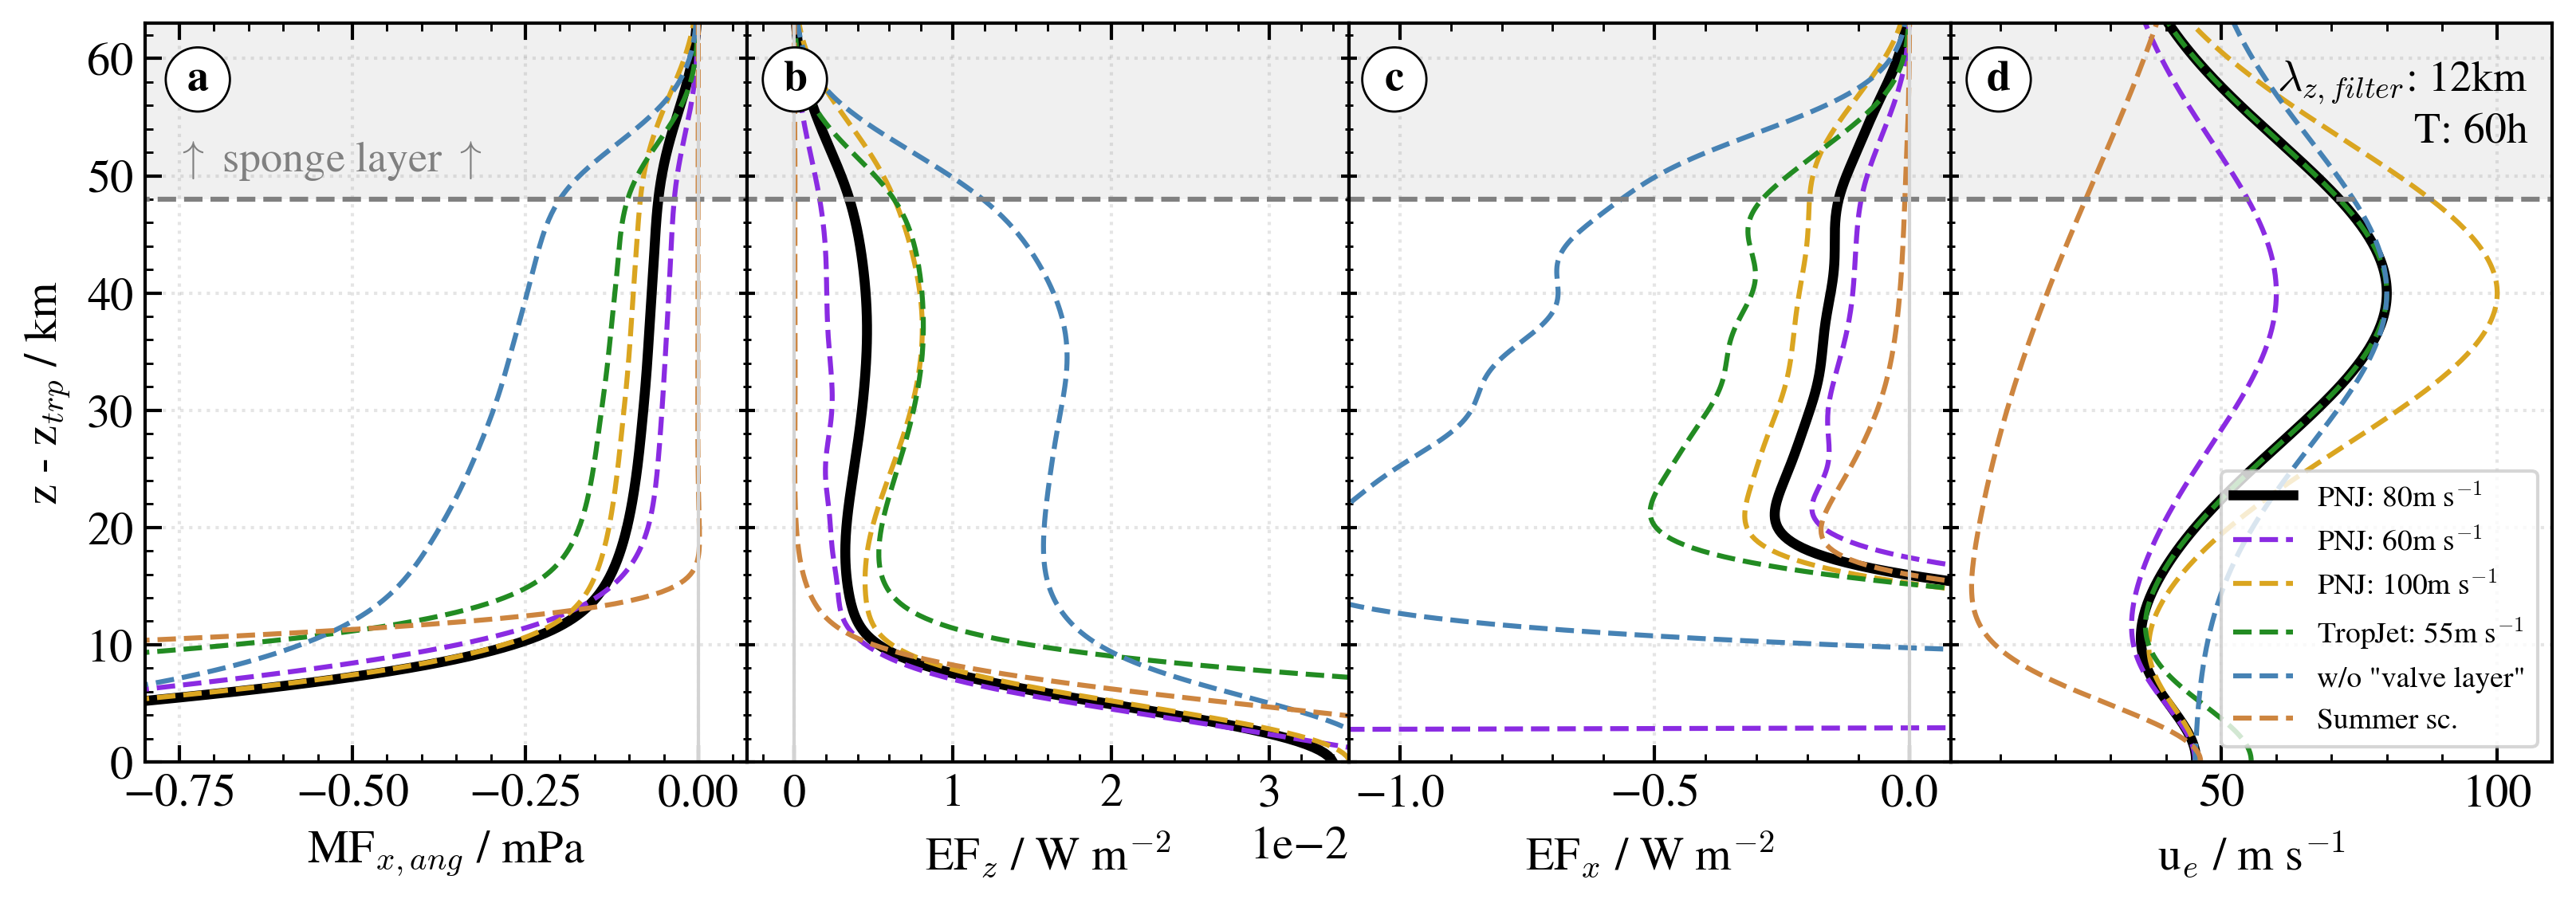
\includegraphics[width=0.99\textwidth]{figures_q3D/TD-zprofiles-translbq3D_wind-T60h-avg.png}
    \caption{Similar to Figure \ref{fig:q3D_shape}, but simulations utilze different wind profiles as indicated in (d). All other parameters of the simulations are identical to the reference simulation.}
    \label{fig:q3D_wind}
\end{figure*}
The main focus of this section is on the comparison of different ambient wind profiles presented in Figure \ref{fig:q3D_wind}d. A brief discussion of simulations with varying Coriolis parameter and stratification is found at the end.

The dashed purple and yellow lines in Figure \ref{fig:q3D_wind} represent simulations with a weaker ($u_{PNJ,max}$=\SI{60}{\meter\per\second}) and stronger ($u_{PNJ,max}$=\SI{100}{\meter\per\second}) PNJ. The tropopause jet (TPJ) at lower altitudes is the same for these simulations. As expected, momentum and energy fluxes look almost identical up to approximately $z$=\SI{15}{\kilo\meter}, but deviate in the upper stratosphere. Stronger winds lead to stronger momentum and energy fluxes. An increase of EF$_z$ due to the stronger shear of the PNJ is consistent with the discussion on wind shear and energy production in the previous section, but higher momentum fluxes are caused differently. As derived in the model validation section \ref{sec:linear-MWs} the vertical flux of angular momentum MF$_{x,ang}$ should be similar for all simulations with the same forcing at tropopause level and for conservative wave propagation. Here, the propagation of waves is not conservative due to the negative shear above the TPJ and the resulting wind minimum at $z$=10-\SI{12}{\kilo\meter}. In this so-called "valve layer" nonlinear processes irreversibly dissipate momentum and influence the momentum flux above (\cite[]{kruse_midlatitude_2016}). A close observation of the three relevant wind profiles reveals that the negative shear and the wind minimum of the valve layer is more pronounced for the weaker PNJ (dashed purple line). Therefore, more momentum is attenuated and MF$_{x,ang}$ becomes smaller in the upper stratosphere.

\begin{figure*}[t]
    \centering
    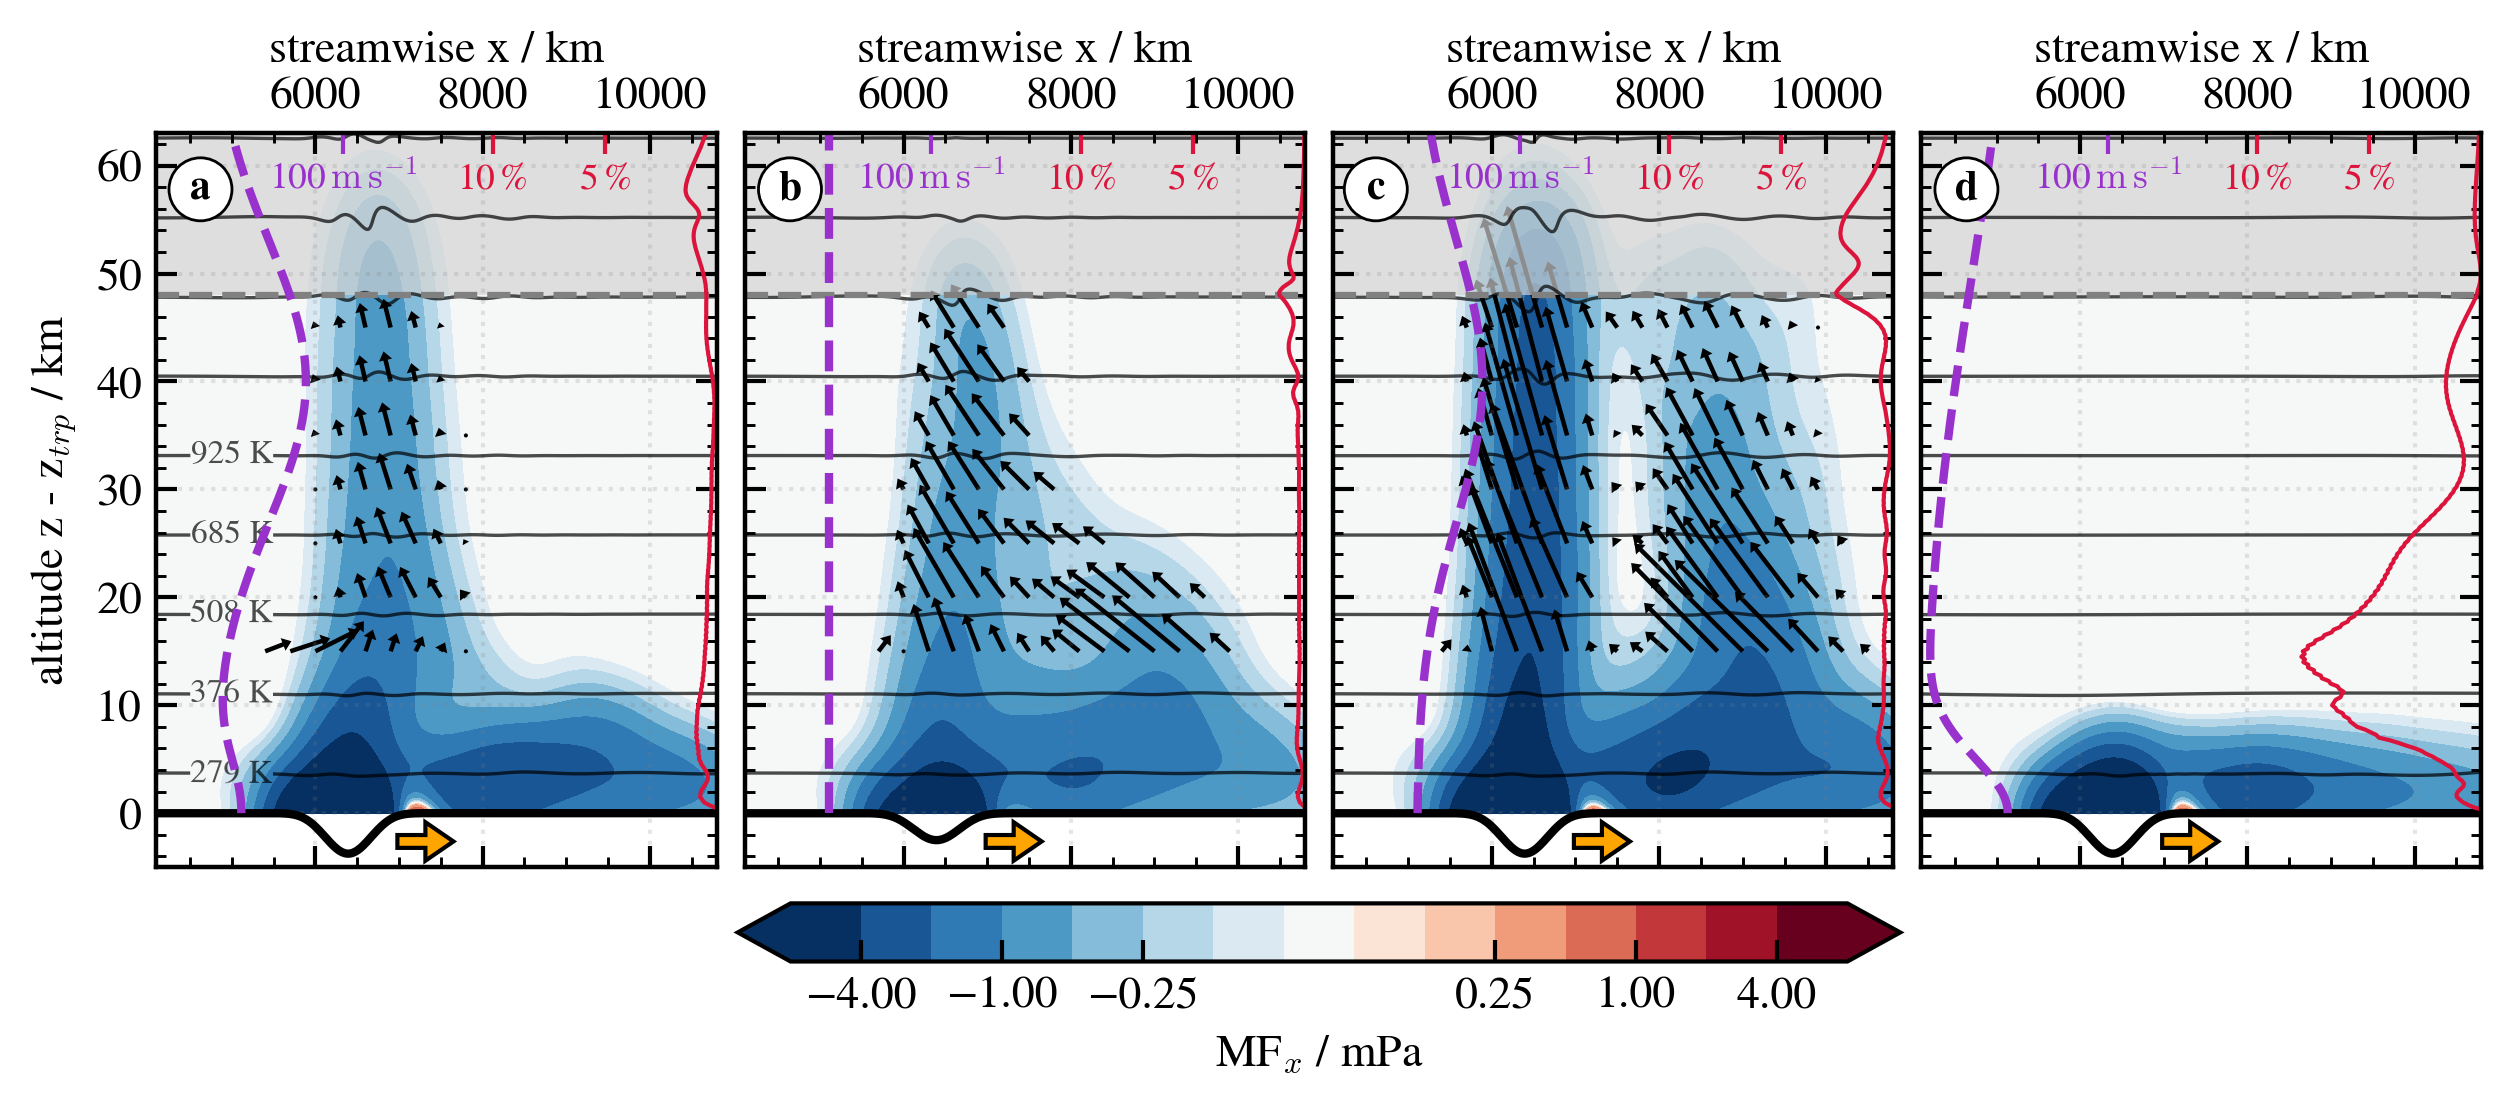
\includegraphics[width=0.99\textwidth]{figures_q3D/Q3D-MFx-towers.png}
    \caption{Cross sections at y=0 and t=\SI{60}{\hour} showing the vertical flux of zonal momentum (MF$_x$) for four different simulations. (a) is the reference simulation, (b) has a stronger PNJ with $u_{max}=\SI{100}{\meter\per\second}$, (c) has no valve layer (wind minimum above the tropopause jet) and (d) represents the summer scenario without a PNJ. Fluxes are averaged with a Gaussian filter according to \textcite[]{kruse_gravity_2015} and black arrows indicate the normalized vector of the energy flux \textbf{EF}.}
    \label{fig:q3D-mfx-towers}
\end{figure*}
The effect of the valve layer becomes much more apparent when comparing the reference simulation to a simulation without a valve layer (dashed blue lines) and the summer scenario for the southern hemisphere stratosphere (dashed red lines in Figure \ref{fig:q3D_wind}). For the blue simulation, maximum speeds of the TPJ and PNJ stay the same, but the valve layer has been removed. For the red simulation, the PNJ is removed and the wind minimum is further reduced, but the wind speed at tropopause level is still the same as in the reference simulation. The momentum and energy fluxes present a consistent picture. Removing the valve layer results in far bigger momentum and energy fluxes compared to all other simulations, removing the PNJ and further decreasing the wind speed of the valve layer leads to vanishing fluxes in the upper stratosphere. Vertical cross sections of MF$_x$ for these simulations further illustrate these features in Figure \ref{fig:q3D-mfx-towers}. In simulations (a) to (c) large values of MF$_x$ reach high up into the upper stratosphere, but for the summer scenario in (d) MF$_x$ disappears above $z$=\SI{10}{\kilo\meter}. \textcite[]{kruse_gravity_2015} called these patterns of high-reaching momentum flux in (a),(b) and (c) flux towers and, again, in the simulation without a valve layer in (c) the tower is much more pronounced compared to the reference simulation (a) or the simulation with a stronger PNJ (b). How can we explain these different flux towers and varying profiles of MF$_{x,ang}$, if linear theory expects vertical vaariations of momentum flux only in the context of critical levels or reflection layers (\cite[]{booker_critical_1967}, \cite[]{jones_propagation_1967} and \cite[]{broad_linear_1995})? \\
At first, we note that wave reflection in the presence of the PNJ is only relevant for horizontal wavelenghts below 30-\SI{40}{\kilo\meter} and can be ruled out for the scales of GWs above tropopause folds (\cite[]{gill_atmosphere-ocean_1982} or \cite[]{mixa_nonlinear_2021}). Furthermore, a slight decrease of MF$_{x,ang}$ with height is already observed for EULAG simulations with a constant wind profile in Section \ref{sec:linear-MWs}, but the decrease observed in simulations of this section with vertical shear is much more pronounced and suggests the presence of critical levels. In a 2D flow an internal GW reaches its critical level $z_c$ when its horizontal phase speed is equal to the background wind. In a 3D rotating fluid with purely zonal background flow (V=0) a critical level is defined for 
\begin{equation}
    \omega - Uk = \hat{\omega} = f,
    \label{equ:critical_level}
\end{equation}
so the intrinsic frequency $\hat{\omega}$ does not vanish, but approaches the Coriolis frequency $f$ and the GW becomes an inertial oscillation (\cite{jones_propagation_1967}). At the same time, the vertical wavelength and group velocity of the GW decrease to 0 at $z_c$ (e.g. \cite[]{lin_mesoscale_2007}). Based on the results from Section \ref{sec:q3D-speed} the horizontal phase speed of NOGWs above propagating tropopause depressions is not 0 as for stationary MWs, but equal to the propagation speed of the depression $c_{p,x}=c_{tf}=\SI{13.88}{\meter\per\second}$. In other words, GWs propagate like MWs within the moving reference frame of the depression. Consequently, the vertical wind profile of the summer scenario in Figure \ref{fig:q3D_wind} and \ref{fig:q3D-mfx-towers} clearly contains a critical level for the excited GWs (wind speed drops below $c_{tf}$) and it is plausible that the flux tower completely disappears in Figure \ref{fig:q3D-mfx-towers}d. However, the wind minimum of the reference simulation or the simulation with an increased PNJ is approximately \SI{35}{\meter\per\second}, so much greater than the wind speed at a critical level, which would be slightly higher than $c_{tf}$. Now, one way to interpret the momentum flux variation with height in these simulations is the valve layer mentioned above. Though linear theory predicts wave dissipation only at the critical level $z_c$, in reality, it takes an infinite time for a GW to actually reach its critical level, because its vertical group velocity and vertical wavelength vanish. Therefore, GW dissipation due to a critical level could be understood as a continuous process that starts as soon as a GW approaches its critical level. In the case of MWs or NOGWs above tropopause depressions, a decreasing background wind with height is synonymous to approaching a critical level, which is consistent with \textcite[]{kruse_midlatitude_2016}'s description of a valve layer: A layer of reduced wind speed with no wind reversal or critical level. \\
\textcite[]{bretherton_propagation_1966} or \textcite[]{booker_critical_1967} conclude from their analysis (W.K.B approximation) that the flow regime and processes effecting the momentum and energy fluxes can be related to the gradient Richardson number $R_i=\frac{N^2}{\frac{\partial U}{\partial z}}$, but admit that their linear analysis is limited in the vicinity of critical levels. A few years later, nonlinear numerical simulations by \textcite[]{breeding_non-linear_1971} revealed three flow regimes for $R_i \leq \frac{1}{4}$, $\frac{1}{4} < R_i < 2$ and $R_i \geq 2$.
\begin{wrapfigure}{r}{6cm}
    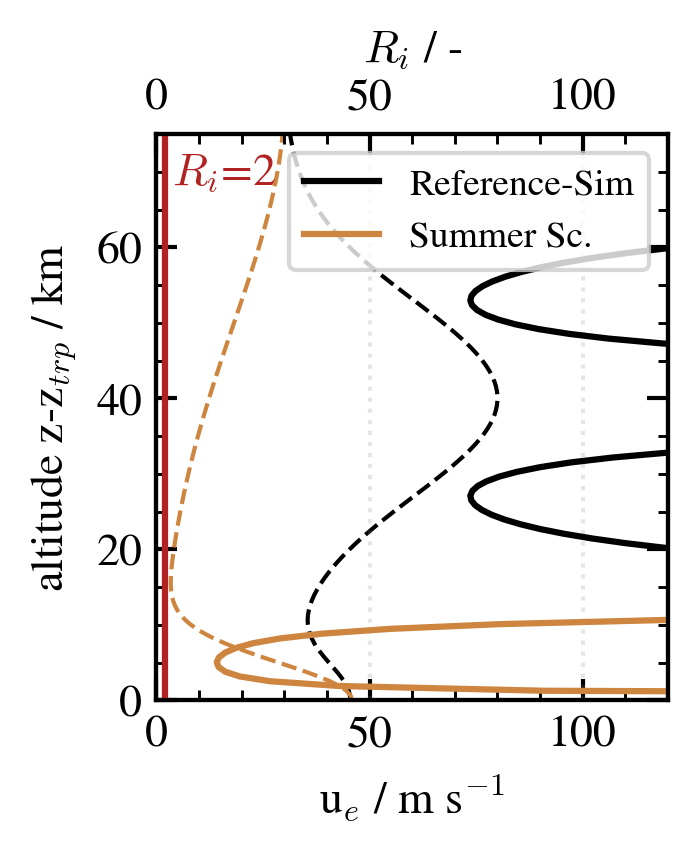
\includegraphics[width=6cm]{figures_q3D/critical-layer-ana.png}
    \caption{Wind profiles (dashed lines) and Richardson number $R_i$ (solid lines) for the reference simulation (black) and the summer scenario (reddish). The vertical red line indicates $R_i=2$.}
    % \vspace{-110pt} % This removes the white box on the second page
    \label{fig:ri}
\end{wrapfigure}
For the latter, very little of the GW penetrates through the critical level and almost all of the wave's energy and momentum is reabsorbed by the mean flow without necessarily invoking turbulence or other dissipative processes (\cite[]{booker_critical_1967}). Figure \ref{fig:ri} illustrates that $R_i >> 2$ holds for all levels of the reference simulation and the summer scenario with a much stronger negative shear above the TPJ, so we can conclude that the valve layer (negative shear above the tropopause jet) is responsible for decreasing MF$_{x,ang}$ in Figure \ref{fig:q3D_wind} due to absorption of energy and momentum by the mean flow.  

A last variation of the ambient wind profile in Figure \ref{fig:q3D_wind} is a stronger TPJ (green dashed lines). The wind speed at tropopause level is increased by \SI{10}{\meter\per\second}, but the wind minimum above is almost similar to the reference simulation. As expected, MF$_{x,ang}$ is larger in the lower stratosphere, but it is also more pronounced in the upper stratosphere. Though the negative shear above the TPJ is stronger, more momentum can pass through the valve layer. The momentum flux in the upper stratosphere is also higher compared to the simulation with a stronger PNJ (dashed yellow line in Figure \ref{fig:q3D_wind}), but a higher energy production in the positive shear of the PNJ compesates for the smaller momentum flux. Increasing the TPJ by \SI{10}{\meter\per\second} had exactly the same effect on upper level EF$_z$ as increasing the PNJ by \SI{20}{\meter\per\second}. From a quantitative point of view, GW activity in the upper stratosphere seems to be more sensitive to the ambient wind at excitation level (tropopause) as to the flow at upper levels.

Simulations with varying Coriolis parameter or stratification have also been conducted, but not presented in the figures. When decreasing the Coriolis parameter, so it corresponds to a latitude of \SI{45}{\degree S}, all momentum and energy fluxes increase and we observe a lower transition from positive to negative values for EF$_x$. On the contrary, reducing the Brunt-Väisälä frequency to $N=\SI{0.015}{\per\second}$ leads to marginal changes in the momentum and energy fluxes, because density and potential temperature profiles are coupled in the Bacmeister-Schoeberl model.

%%%%%%%%%%%%%%%
% However, these changes in the wind are centred above the critical level, so that the change in the wind has only a small effect on the height of the critical level

% Thus the packet is neither transmitted nor reflected - it simply slows down until either viscosity, turbulence or other non-linearities destroy it as a coherent entity.

% kruse 2016
% Such a layer might allow small-amplitude mountain waves to be trans- mitted unaffected but might also cause larger-amplitude mountain waves to steepen, become nonlinear, and attenuate 

% Another view relates energy fluxes and valve layer  via group velocity also slows down the GW propagation (reduces group velovcity)

% \cite[]{dornbrack_evidence_2002} waves over scandinavia
% convective instability vs. shear instability 

% 3D critical levels!! \cite[]{teixeira_momentum_2009}
% However, the interest for flows with directional shear and critical layers (where the wave momentum is deposited over a continuous range of heights, as opposed to critical levels) has increased recently, since these flows are much more realistic

% For a directionally sheared flow and a 3D mountain, there is no single critical level, but a distribution of them with height, depending on the wavenumber of the gravity waves (i.e., a critical layer). This study aims to calculate the momentum flux in such situations of directional shear and 3D orography, addressed first by SG99

% According to Eliassen and Palm [1960] for linear, steady, small-amplitude, non-dissipative MW

% Fritts 2003
%Dissipation results from processes such as radiative damping [Fels, 1984; Zhu, 1994], wave–wave and wavemean flow interactions [Broutman and Grimshaw, 1988; Sutherland, 2000, 2001], and wave breaking and instability processes (see section 6).
%%%%%%%%%%%

%%%%%
% Vertical wavelenghts increase proportional to zonal cross sections and energy fluxes increase for stronger wind

% \begin{equation}
%     c_{gx} \approx \frac{N^2 \alpha}{m \sqrt{f^2+N^2 \alpha^2}} \approx \SI{-26.9}{\meter\per\second} 
% \end{equation}
% with a negative $m$ for upward propagating waves and the vertical group velocity
% \begin{equation}
%     c_{gz} \approx -\alpha c_{gx} \approx \SI{0.36}{\meter\per\second}
%     % \label{equ_lid:cgz}
% \end{equation}
%
% \section{Influence of Coriolis force and stratification}
% \begin{figure*}[t]
%     \centering
%     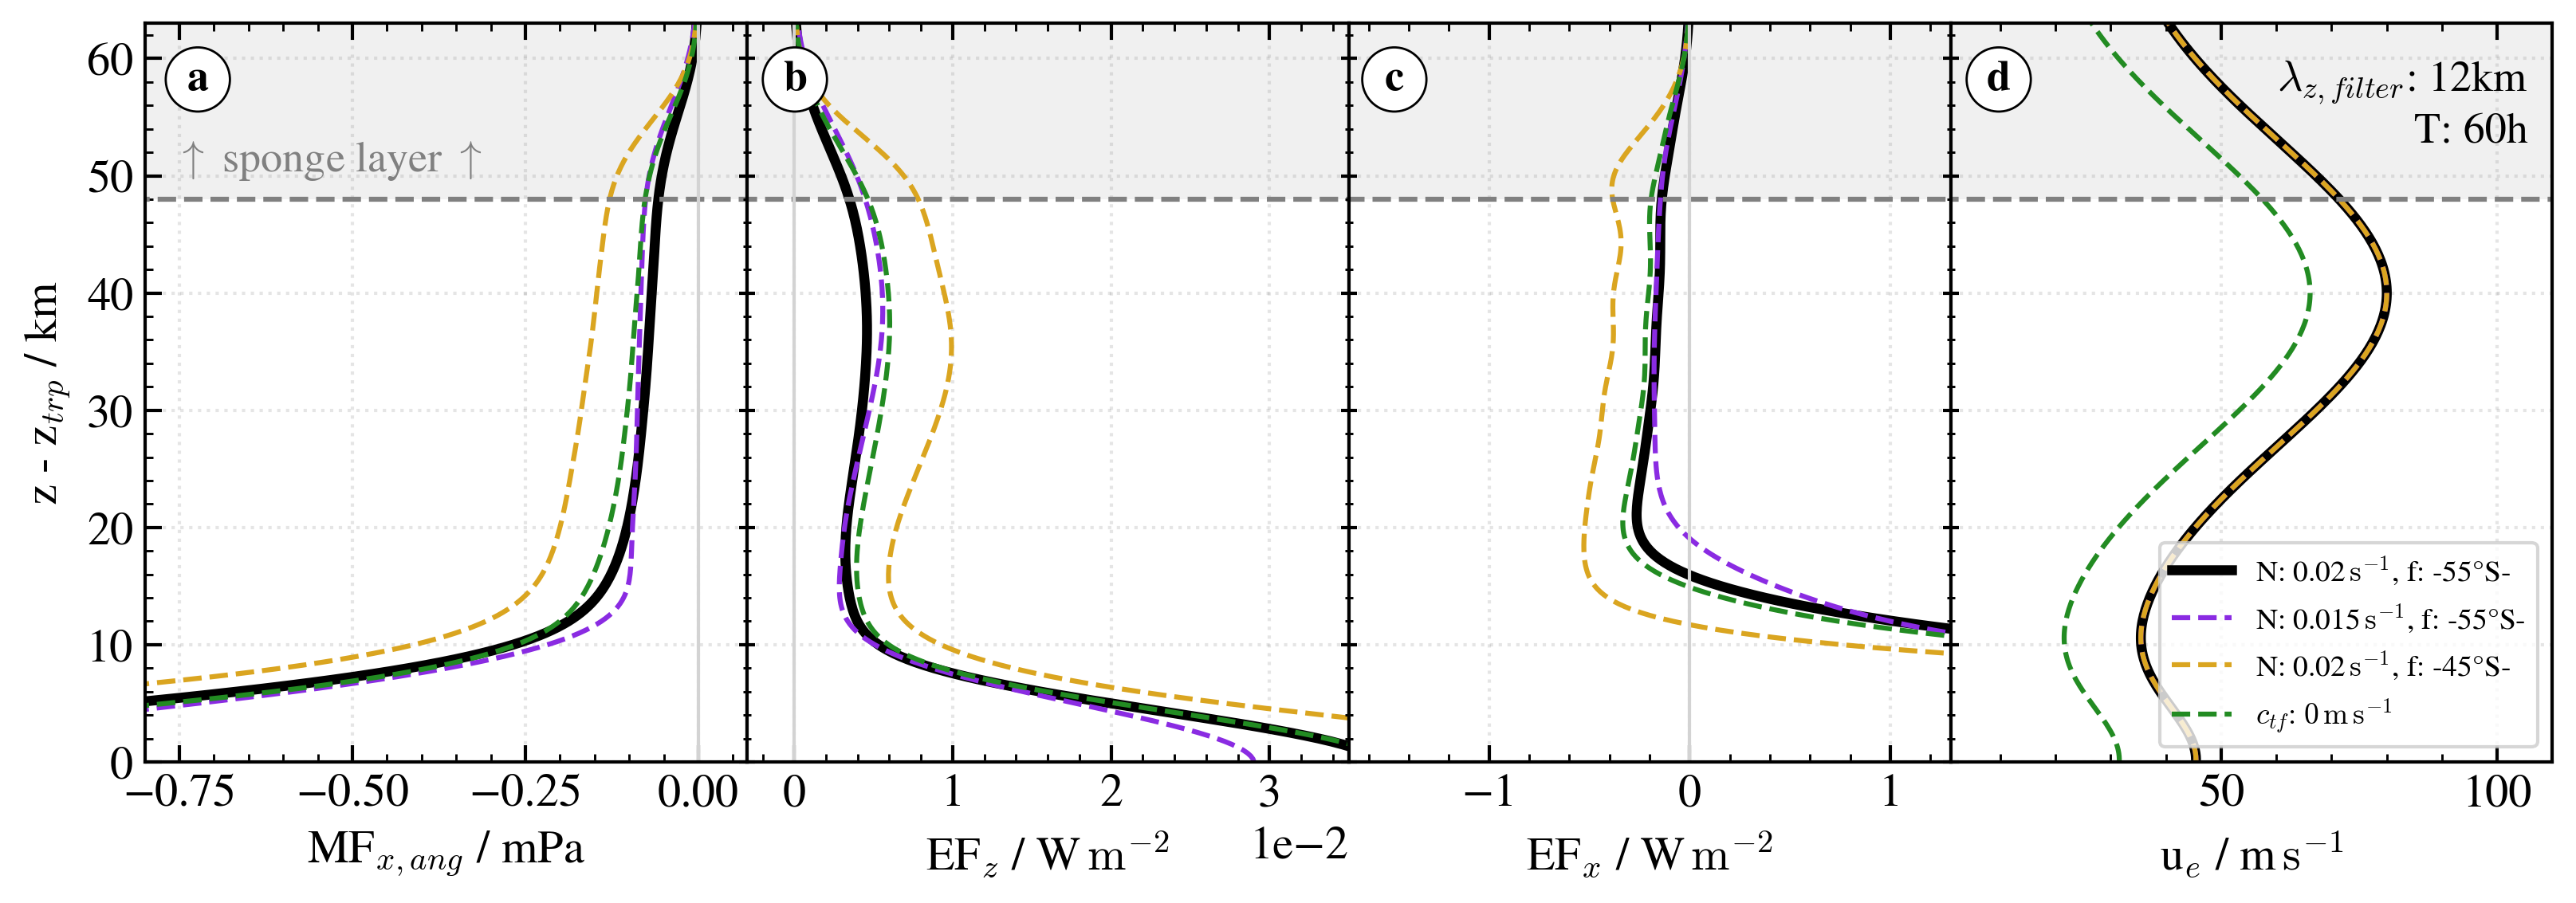
\includegraphics[width=0.99\textwidth]{figures_q3D/TD-zprofiles-translbq3D_atm-T60h-avg.png}
%     \caption{Similar to Figure \ref{fig:q3D_shape} and Figure \ref{fig:q3D_wind}, but simulations vary the Coriolis paramter $f$, the Brunt-Väisälä frequency $N$ and the propagation speed $c_{tf}$. All other parameters of the simulations are identical to the reference simulation.}
%     \label{fig:q3D_atm}
% \end{figure*}

\section{Summary and answer to research question (R1)}
\label{sec:q3D-summary}
The objective of this chapter was to identify zonal and vertical properties of the tropopause (width and height of a depression) and the stratospheric environment (e.g. variation of the ambient wind profile) that significantly influence the GW activity in the upper stratosphere to answer the research question
\begin{tcolorbox}[]
    (R1) How sensitive are NOGWs from propagating tropopause depressions to the depression's 2D shape and to 2D properties of the stratospheric environment?
    % How are NOGWs effected by ...
    % (R2) How sensitive are NOGWs from propagating tropopause folds to the 2D shape of the depression and the stratospheric environment?
\end{tcolorbox}
Under the assumption that the tropopause can be emulated by a transient, impermeable and frictionless lower boundary in the numerical simulations, a fundamental result of the analysis came out of Section \ref{sec:q3D-speed}. Varying the propagation speed of the tropopause depression $c_{tf}$ has a similar effect as varying the whole vertical profile of the ambient wind. So NOGWs above tropopause depressions behave and propagate just like MWs within the reference frame of the propagating depression for a relative wind $u_{e,MW}$ (Equation (\ref{equ:MW_forcing})). \\
Furthermore, the presented simulations suggest the following qualitative conclusions for the sensitivity of NOGWs excited above propagating tropopause depressions:
\begin{itemize}
    \item Naturally, the GW activity in the upper stratosphere is proportional to the depth $H$ and inversely proportional to the half width $L$ of the tropopause depression.
    \item GW activity also increases for a stronger background wind speed $u_e(z)$ with a higher sensitivity for wind speeds in the lower stratosphere (tropopause jet) compared to the PNJ higher up.
    \item A pronounced stratospheric wind minimum has the largest effect on upper stratosphere GW activity (valve layer-like effect). Removing the valve layer without increasing the maximum wind speeds of the jet streams increases the GW activity in the upper stratosphere the most. 
    \item Introducing weak winds above the tropopause jet (summer scenario of southern hemisphere stratosphere) completely suppresses GW activity in the upper stratosphere. GWs already dissipate at lower levels due to a critical level that exists for $u_e \leq c_{tf}$.
    \item Decreasing the Coriolis force enhances the GW activity in the whole stratosphere.
\end{itemize}
Another informative test could be the variation of the vertical width $\sigma$ in Equation \ref{equ:wind-distribution} of the TPJ or the PNJ to increase (or decrease) the vertical shear without removing the valve layer completely, but it is omitted within the framework of this thesis. \\
The simulations presented in this chapter were conducted in 3D to correctly incorporate the Coriolis force. However, ambient conditions like the background wind were constant in meridional direction, so these simulations basically describe a scenario with the PNJ directly centered above the tropopause depression. In reality, the PNJ is often observed south of the storm track and corresponding tropopause folds during austral winter. The analysis in the next chapter deals with this situation and investigates the impact of meridional properties on the GW activity in the upper stratosphere.